%% -*- coding: utf-8 -*-
\documentclass[12pt,pagesize,paper=192mm:108mm,landscape]{scrbook} 
%1920x1080 1280x720
\areaset[current]{192mm}{108mm}
\usepackage{calc}
\usepackage[T2A]{fontenc}
\usepackage[utf8]{inputenc}
\usepackage[english,russian]{babel}
\usepackage{microtype}
\usepackage{misccorr}
\usepackage{cmap}
%\usepackage[unicode=true]{hyperref}
\usepackage{graphicx}
\usepackage{amssymb}
\usepackage{amsmath}
%\usepackage{srcltx}
\usepackage{textcomp}
\usepackage{xspace}
%научные символы и смайлики \smiley \frownie
\usepackage{wasysym}
\usepackage{ccicons}
\begin{document}
\begin{titlepage}
  \vspace*{-0.5em}
  \begin{center}    
    \hspace*{3em}
    \begin{minipage}[t]{1.5em}
      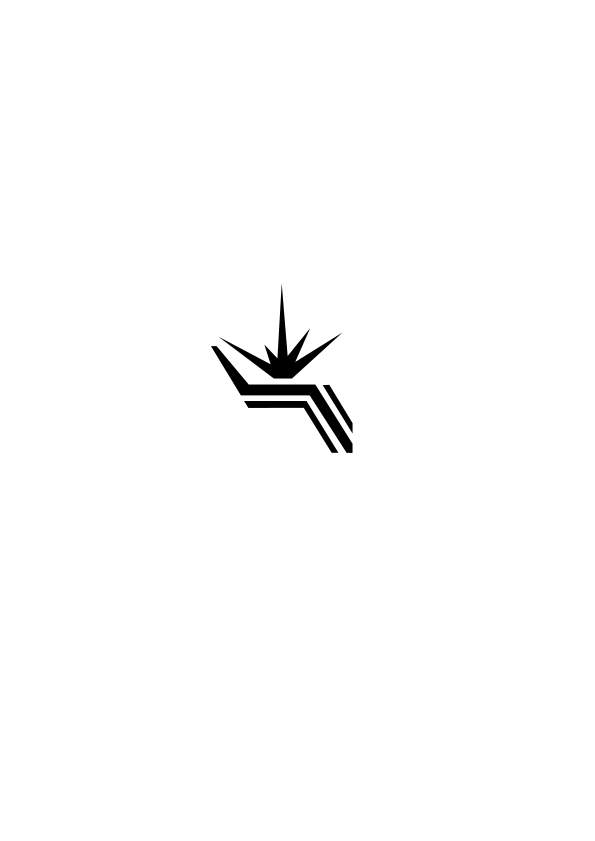
\includegraphics[width=\textwidth]{../BINP-logo}
    \end{minipage}\hfill
    \begin{minipage}{0.115\linewidth}
    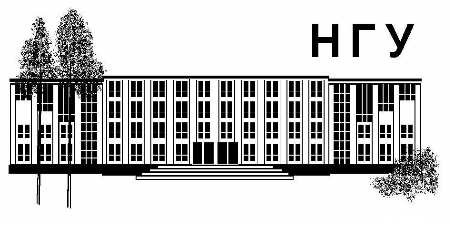
\includegraphics[width=\textwidth]{../NSU-logo}
    \end{minipage}
    \hfill
    \hspace*{4.5em}

    Кафедра теоретической физики физического факультета НГУ
    \medskip

    \Large
    Профессор Грабовский А.\,В.
    \smallskip

    \Large
    \textbf{Дополнительные главы ОТО: чёрные дыры.}
    \smallskip

    \Large
    Лекция № 4
    \vfill

    \normalsize
    \begin{minipage}{0.90\linewidth}
      Изотропные координаты для решения Шварцшильда. Вложение
      многообразия Шварцшильда при $t=\text{const}$,
      $\theta=\text{const}$ в трехмерное евклидово пространство. Мост
      Эйнштейна"--~Розена. Вектор Киллинга $\partial_t$ на
      многообразии Крускала, его орбиты и фиксированные точки,
      области, где он нулевой, времени- и
      пространственно"=подобный. Ось Боера"--~Крускала. Нормаль
      к~гиперповерхности, нулевые гиперповерхности, нормали и
      касательные к ним. Доказательство того, что нормаль к~нулевой
      гиперповерхности как вектор касательной определяет геодезическую
      на этой поверхности. Генераторы нулевых
      гиперповерхностей. Горизонт Киллинга. Поверхностная гравитация.
     \end{minipage}
    \vfill

    \normalsize \ccbysa\hspace{0.5em}  Новосибирск 2022
  \end{center}
\end{titlepage}
\end{document}
